\section{Materials and methods}
\label{sec:methods}

\subsection{Research setting and evidence base}

LabAutomation.io is a public specialist forum covering liquid handling, devices, schedulers, open-source tools, integrations, and automation practice \cite{labautomation_about,forum_welcome}. The platform's terms retain contributor rights and restrict automated access and monitoring \cite{labautomation_terms}. The study therefore used manual public-source review and did not perform automated corpus collection. The retained pilot contains 55 purposively selected discussions dated from 2022 through 2026. Selection sought conceptual coverage across platforms, workflow layers, incident types, design discussions, documentation requests, product reports, and positive community outcomes. The sampling frame was constructed for evidence mapping and metric design. It was not constructed to estimate topic prevalence.

The public release records thread title, date, category, source URL, primary code, direct secondary codes, evidence type, public resolution class, public artifact, migration status, evidence strength, and an analytical note. Usernames and profile attributes are excluded. Short quotations are anonymized and linked to their discussion. Public resolution classes distinguish confirmed, partial, open, mixed, product-reported, and migrated outcomes. An open thread does not imply operational non-resolution because the work may have continued elsewhere.

\subsection{Analytical units and episode segmentation}

The thread is an efficient discovery unit and an unreliable universal analytical unit. A long discussion can contain several mechanisms. One version-control discussion moved from portable source files to generated identifiers, physical teaching, active recovery workspaces, and an open integration bridge \cite{forum_tecan_git}. A driver discussion combined commercial access, serial communication, platform-state synchronization, and workaround design. A scheduler comparison combined device breadth, deployment effort, training, licensing, and scheduling capability \cite{forum_scheduler_feedback}. Treating each as one observation would erase these transitions.

A deliberately difficult subset of 14 threads was therefore segmented into 45 episodes. Each episode records the initiating problem, lifecycle stage, primary technical construct, ecosystem modifiers, evidence form, detectability, consequence, resolution, public artifact, counterexample status, source, and coding note. The subset was selected to stress the taxonomy through multi-construct threads, incidents, product reports, vendor participation, and positive outcomes. It does not constitute an independent sample. All coding was performed by one analyst. The study reports no inter-rater statistic and describes the output as a single-coder pilot. Reliability is approached through explicit boundary rules, hard-case adjudication, retained counterexamples, executable value checks, and a publication claim ledger. The prepared adjudication set is released as \path{data/derived/reliability_subset.csv}, which names the expected primary code, the most plausible competing code, and the specific adjudication question for each thread in the difficult subset so that an independent coder can repeat the hardest decisions without renegotiating the coding task.

\begin{figure}[t]
  \centering
  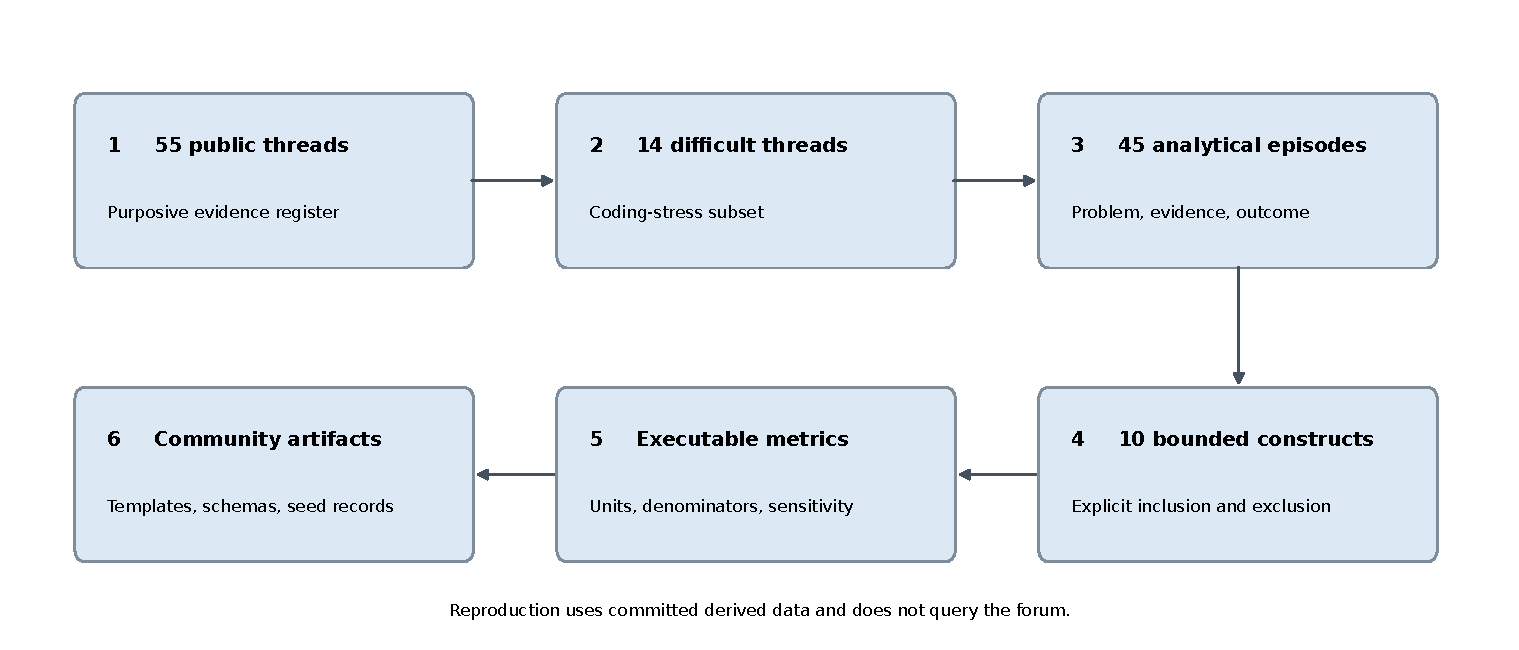
\includegraphics[width=\linewidth]{figures/study_workflow.pdf}
  \caption{Analytical workflow. The public release contains derived records and does not reproduce a full forum corpus.}
  \label{fig:workflow}
\end{figure}

\subsection{Taxonomy construction}

The taxonomy contains ten constructs. B1 and B10 are ecosystem conditions and enter as primary codes only when knowledge governance, documentation, training, or support is the central object. B2 through B4 concern interfaces and representations. B5 through B7 concern runtime coordination. B8 concerns evaluation semantics. B9 concerns AI-specific context and feedback. Each code has inclusion rules, exclusion rules, primary-code eligibility, adjacent codes, required evidence, and a boundary test.

\begin{figure}[t]
  \centering
  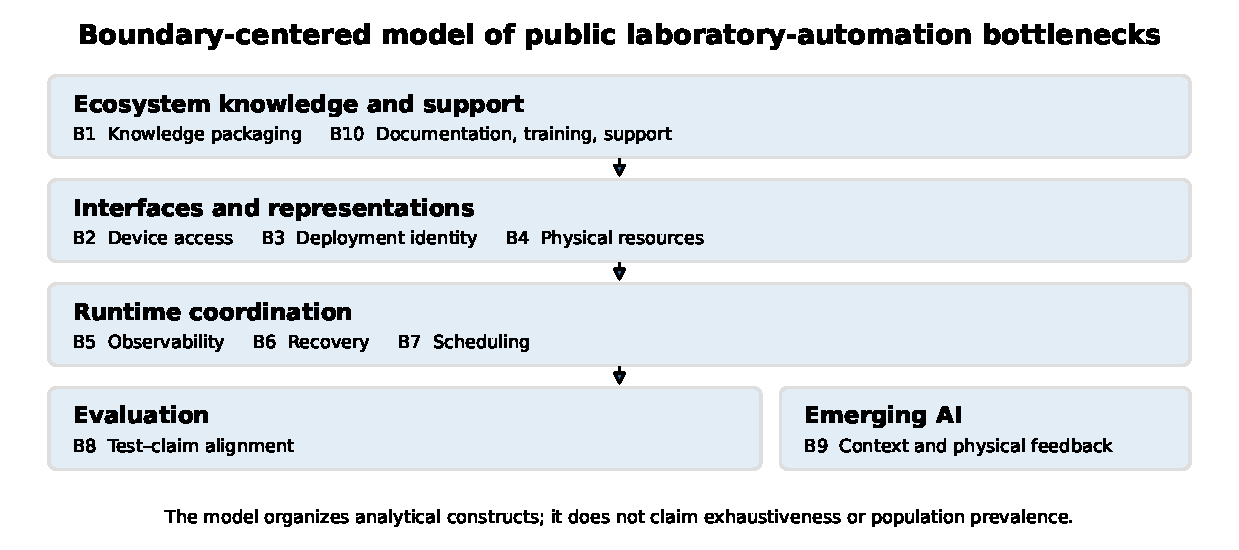
\includegraphics[width=\linewidth]{figures/conceptual_model.pdf}
  \caption{Layered taxonomy and boundary-centered interpretation. The structure organizes the pilot evidence and remains revisable.}
  \label{fig:conceptual-model}
\end{figure}

The coding process retained positive and negative cases. A plate-reader integration released a public API, example, and contribution path. A tip-definition incident produced a cross-machine post-mortem and merged corrections \cite{forum_tip_postmortem}. A documentation thread exposed a low-friction edit pathway \cite{forum_plr_docs}. A bounded abort-handler example demonstrated material recovery under a specified software-error scenario \cite{forum_return_volume}. These cases prevent the taxonomy from becoming a catalogue of closure or failure.

\subsection{Bounded metrics}

The metrics use units that can be defined from public technical evidence.

\paragraph{Integration Accessibility Score.}
A device--interface pair is scored over documentation, API or protocol access, licence clarity, simulator or isolated testing, examples or reference implementation, and identifiable maintenance or support. Components take values 0, 0.5, or 1. Unknown is excluded from the component mean and reported separately. The score measures public accessibility conditions, not device reliability.

\paragraph{Reproducibility Manifest Completeness.}
A deployment object is evaluated over applicable fields including method source, libraries, labware definitions, liquid classes, deck layout, teaching or calibration, drivers, software or firmware, checksums, and runtime initialization. A score of 1 requires explicit immutable binding, 0.5 indicates discussion or partial representation, and 0 indicates omission from the reviewed evidence.

\paragraph{Physical Definition Completeness and evidence grade.}
A resource definition is scored over identity, external and internal geometry, material, tolerance, coordinate semantics, nesting, operating properties, provenance, device validation, and independent reproduction. A separate ordinal evidence grade distinguishes unspecified, declared, measured, device-validated, and independently reproduced records.

\paragraph{Observability Coverage.}
An execution or diagnostic object is scored over linked run and configuration identity, material or resource identity, command, acknowledgement, physical observation, modeled state change, warning or failure, human intervention, recovery, and final result or disposition. Raw log volume is not part of the score.

\paragraph{Preflight Preventability Rate.}
A partial-execution scenario is eligible when at least one physical action completed before failure. A scenario is preflight preventable when the failure could be detected from information available before the first irreversible action. Indeterminate cases remain separate. Complete-case estimates and conservative and optimistic sensitivity bounds are reported.

\paragraph{Constraint Completeness.}
A scheduling scenario is decomposed into resource identities, tasks, durations, transfers, release times, precedence, resource eligibility, timing windows, sample stability, interruptibility, terminal disposition, priorities, and failure policy. Opening completeness, missing-field discovery, and scenario-specific resolution are distinct measures.

\paragraph{Test--Claim Alignment.}
Each bounded claim is scored over test object, environment, acceptance criterion, observed evidence, and claim scope. Fully aligned claims require all five elements to support the normalized statement. Partial claims retain useful evidence and require narrower wording.

\paragraph{Context Expansion Ratio.}
An AI-method discussion is segmented into opening context classes and reply-added material classes. Core execution and broader deployment ontologies are reported separately, along with a conservative grouping that merges related classes. The ratio is a requirements-elicitation measure and is not a model error rate.

\subsection{Relationship analysis and sensitivity}

All 28 pairwise relationships among B2--B9 were computed from the 55-thread direct-support matrix. For codes $A$ and $B$, the analysis reports overlap, Jaccard similarity, lift, the phi coefficient, conditional probabilities, and a descriptive risk ratio. A pilot attention threshold of $\phi\geq0.30$ and lift $\geq1.50$ identifies relationships for qualitative adjudication. The threshold is a prioritization rule and has no inferential interpretation.

One-thread recoding sensitivity was calculated by holding marginal counts fixed and decreasing or increasing overlap by one where logically possible. Each leading relationship was then assessed for construct independence, a proposed mechanism, alternative explanations, counterexamples, a prospective metric, and a falsification criterion. Documentation burden and interface accessibility were also compared in five matched cases. Because the instruments share documentation, access, examples, and support components, that analysis is classified as convergent validity and not as a causal test.

\subsection{Claim control and reproducibility}

The publication claim ledger records each proposed statement, claim class, evidence source, denominator, safe wording, prohibited overclaim, sensitivity, and status. The executable repository recomputes headline values from committed CSV and YAML artifacts. Tests assert corpus size, field-level means, bounded metrics, Wilson intervals, association values, and schema validity. The retained workbook provides provenance; ordinary reproduction uses committed derived files and does not contact the forum.
